\section{Power Percent Reactor}
\label{sec:pp_reactor}

The \gls{nrc} publishes a daily Power Reactor Status report for each reactor operating under its jurisdiction \cite{nrc_power_2025}. These reports contain, amongst other things, a report of the percentage of the total power capacity at which the operators say the reactor operated. In the case of a fuel cycle simulation containing a small number of reactors or a full fleet simulation over a short time period, the differences in the power predicted by the \cycamore reactor and reality can diverge.

Figure \ref{fig:pp_full} we examine the single reactor operating at the Clinton Clean Energy Center, with a reference unit power capacity (i.e., net power) of 1062 MWe according to the \gls{iaea} \gls{pris} database \cite{IAEA_PRIS}, and compare it to the results from the \cycamore reactor modeled over the same time frame. This figure excludes the startup of the \cycamore reactor, which we set several months before this window to ensure that it was operating on the same schedule as the data from the \gls{nrc} suggest the real reactor was operating on from the start of 2021 through the end of 2024.

\begin{figure}
  \centering
  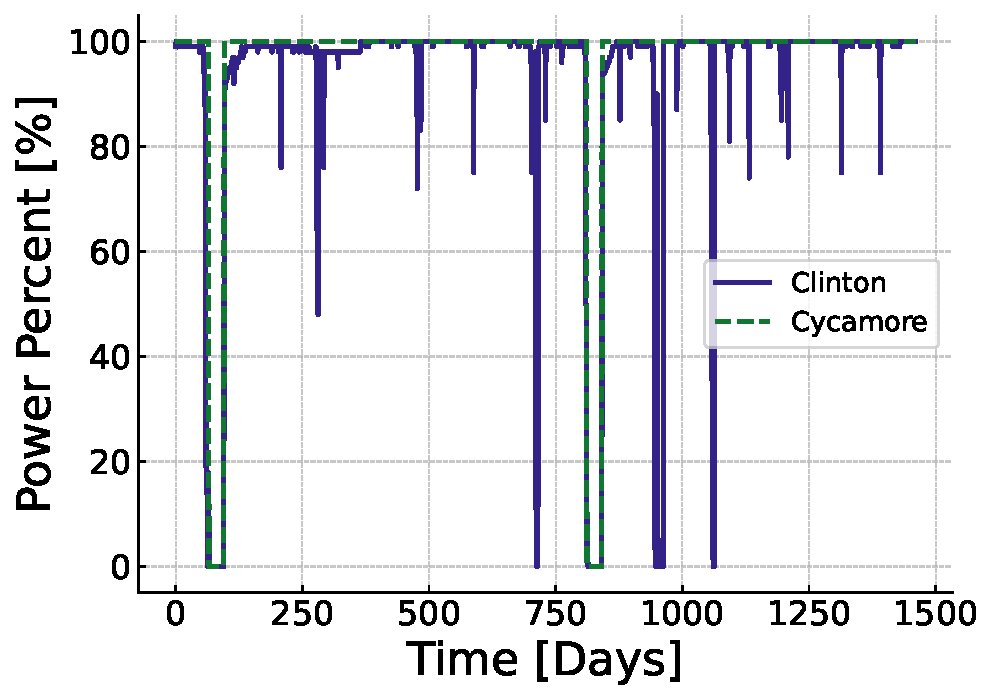
\includegraphics[scale=0.7]{images/power_reactor/power_percent_clinton_fake.pdf}
  \caption{Clinton reactor daily power percent 2021-2024}
  \label{fig:pp_full}
\end{figure}

Performing a simple numerical integration, we find that the total energy produced by both reactors differ by just under 51 GWe with a percent difference of 3.52\%. These differences can be negated by comparing to a base case in the simulation, but for the purposes of our hypothetical small scale model users might be interested in incorporating realistic fluctuations in power and find that the two scenarios in Figure \ref{fig:pp_full} were not equal on 908 days, or 62.2\%, of the 1460-day simulation.

